%UNLIKE IN A REGULAR TEX FILE, DON'T PUT ANY PREAMBLE MATERIAL HERE
\section*{Abstract}
We present preliminary studies into the development of efficient and effective strategies for the usage of LSST in optical follow-up of gravitational wave events detected by the Advanced LIGO and Virgo interferometers. Specifically, we focus on the detection and characterization of kilonovae across a wide range of ejecta properties and composition. We show that for the main LSST survey (RESULTS). In contrast, focused target-of-opportunity follow up with an investment of N minutes per night for M nights allows (OTHER RESULTS). We find that (MORE RESULTS). Something about using LSST for TOO stuff.

\clearpage
\section{Introduction}
\label{sec:ch6_intro}
The discovery of an optical counterpart associated with the the binary neutron star merger GW170817 was a watershed moment in the development of joint gravitational wave and electromagnetic (GW-EM) astronomy \citep{LIGOGW170817,LIGOMMAPaper,Arcavi+17,Coulter+17,GW170817DECam,Valenti+17}. Subsequent modeling of the optical light curves revealed behavior consistent with that of a kilonova \citep{Cowp+17,Kilpatrick+17,Tanaka+17,Villar+17b, Tanaka+18}, an optical/NIR transient expected to accompany compact object mergers involving at least one neutron star \citep[for a review see e.g.,][]{Metzger2017}. The discovery of this optical transient has opened up numerous new and exciting science possibilities. These include studies into the host galaxy \citep[NGC4993, see e.g.,][]{Blanchard+17,Cantiello+18}, constraining the neutron star equation of state \citep[see e.g.,][]{Radice+18}, and even making independent measurements of the local Hubble Constant \citep[H$_0$, see e.g.,][]{LIGOH0,Guidorzi+17}.

If we wish to build upon the success of GW170817 and push into new realms of joint GW-EM science then we must work to facilitate future detections of both gravitational wave sources {\em and} their associated electromagnetic counterparts. A key component of future searches for gravitational wave events is improving the ability of the interferometer network to localize sources on the sky. Over the next several years, as both Advanced LIGO and Virgo reach their design sensitivity, it is expected that they will be able to localize compact binary mergers to sky areas of approximately tens to hundreds of deg$^2$ \citep{LIGOLocalization,ChenHolz16}. Major improvements to sky localization will continue over the next decade as two additional interferometers, KAGRA in Japan \citep{KAGRA} and LIGO-India \citep{LIGOIndia}, join the network. In this five detector regime, compact binary mergers will be localized to just $\apx10$~deg$^2$ \citep{Fairhurst2014,ChenHolz16}.

Similarly, improving our ability to identify electromagnetic counterparts in these localizations will rely on using the next generation of optical facilities that are soon to be coming online. One such facility, the Large Synoptic Survey Telescope \citep[LSST,][]{Ivezic+09}, will be the premiere time-domain in the Southern hemisphere during the next decade. LSST boasts an 8.4-m primary mirror and a 9.6 deg$^2$ field-of-view. This powerful combination of large aperture and wide field of view makes LSST uniquely suited to the task of gravitational wave follow-up. The field-of-view is particularly well matched to the expected localization regions allowing LSST to observe a high fraction of the localization probability in just one or two pointings.

Of particular importance is the development of efficient and effective strategies for gravitational wave follow-up with LSST. This first involves understanding both the rate and properties of kilonovae detected in the LSST main survey. This was investigated by \citet{Scolnic+18} who injected model light curves of the kilonova associated GW170817 \citep{Cowp+17} into the LSST cadence. They found that LSST should detect $\apx7$ GW170817-like kilonovae per year during the ten year main survey. However, these kilonovae were detected only a few times, leading to poorly-sampled light curves. As a result, real-time identification of modeling of these kilonovae will be difficult. Furthermore, these kilonovae are detected far beyond the sensitivity horizon for LIGO, meaning that an association between these kilonovae and a gravitational wave detection is unlikely. This suggests that triggered target-of-opportunities may be a more promising approach.

Here we expand on the groundwork established by \citet{Scolnic+18} along two new avenues. First, we expand the range of kilonovae models considered in the LSST main survey. This is accomplished by considering a wider range of ejecta masses and composition to fully explore the potential range of kilonovae brightness and timescales. Second, we expand beyond the main survey cadence and explore the detectability of kilonovae in triggered target-of-opportunity follow-up observations. We explore not only the ability of such observations to detect kilonovae, but also identify and characterize their behavior. 

This work is organized as follows: In \cref{sec:ch6_models} we describe the expanded range of kilonovae models used in our simulated observations. In \cref{sec:ch6_obs} we describe our methodology for simulating LSST observations using both OpSim for the main survey and SNANA for target-of-opportunity observations In \cref{sec:ch6_analysis} we present the results of our simulated observations. Lastly, discussions and conclusions are presented in \cref{sec:ch6_conc}.

All magnitudes presented in this work are given in the AB system unless otherwise noted. Cosmological calculations are performed using the cosmological parameters $H_0 = 67.7$ km s$^{-1}$ Mpc$^{-1}$, $\Omega_M = 0.307$, and $\Omega_{\Lambda} = 0.691$ \citep{Planck2016}.

\clearpage
\section{Kilonova Models}
\label{sec:ch6_models}
A kilonova is an isotropic optical/NIR thermal transient produced by the merger of a compact object binary containing at least one neutron star such as a neutron star-neutron star binary (NS-NS or BNS) or neutron star-black hole binary (NS-BH). In either scenario, the merger produces a small amount of ejecta ($\Mej \lesssim 0.1 \msun$), which is typically neutron-rich. As the ejecta expands from nuclear densities, it will synthesize heavy elements via $r$-process nucleosynthesis. These heavy nuclei are unstable and will then decay back to stability. This decay will deposit energy into the ejecta powering the kilonova emission \citep{LP98,Metzger+10,BarnesKasen13,TanakaHotokezaka13,Metzger2017}.

The exact nature of this kilonova emission depends strongly on the composition of the ejecta, specifically the neutron-richness which is parametrized by the electron fraction ($Y_e$). If the material is very neutron-rich ($Y_e \lesssim 0.3$), then the ejecta will undergo strong $r$-process nucleosynthesis, producing very heavy elements ($A > 140$), particularly those in the lanthanide and actinide series. As a result of these heavy elements, the ejecta will have a high opacity $(\kappa \gtrsim 10 \cspg)$. The resulting ``red" kilonova will then be faint with a peak luminosity of $L_p \apx 10^{40}-10^{41} \ergs$, red ($i-z \gtrsim 0$), and exhibit a timescale of $t_p \apx 1$ week \citep{BarnesKasen13,TanakaHotokezaka13}. If instead the material is less neutron-rich ($Y_e \gtrsim 0.3$), then the ejecta will undergo light $r$-process nucleosynthesis, producing Fe-group and light $r$-process elements ($A \lesssim 140$), and the ejecta will have a lower opacity $(\kappa \apx 0.1 \cspg)$. The resulting ``blue" kilonova will be brighter $L_p \apx 10^{41}-10^{42} \ergs$, bluer ($i-z \lesssim 0$), and exhibit a shorter timescale of $t_p \apx 1$ day \citep{Metzger+10,MetzgerFernandez14}.

In practice, the observed kilonova will exhibit some combination of both ``red" and ``blue" features. This behavior was seen in the kilonova associated with GW170817, where the multi-band optical/NIR light curve was best described by a three-component model consisting of ``red"  $(\kappa \apx10 \cspg)$, ``purple"  $(\kappa \apx 3 \cspg)$, and "blue"  $(\kappa \apx 0.1 \cspg)$ $r$-process powered components. This three-component approach was first suggested by \citet{Tanaka+17} as a good approximation to the more complex opacity behavior seen in detailed radiative transport simulations. The three-component approach is also physically motivated as the different emission components may arise from different sources of ejecta present in the merger. The ``blue`` emission may arise from neutron-poor ejecta in the polar region where material is shock-heated during the NS collision \citep{Oechslin+07,Bauswein+13a,Sekiguchi+16} or if the ejecta is irradiated by neutrinos from a long-lived merger remnant \citep{FernandezMetzger13,Just+15,Kasen+15}. The ``purple" and ``red" emission may arise from ejecta produced in the tidal tails during merger \cite{Rosswog+99,Hotokezaka+13} or wind outflows from a post-merger accretion disk \citep{Just+15,SiegelMetzger17}. However, it is currently unknown if the behavior observed in the multi-band light curves of GW170817 will be seen for all kilonovae. For example, if the ``blue" emission is indeed constrained to the polar regions of the ejecta then it will not be observable at all viewing angles, whereas the more isotropic ``red" emission from tidal tails or post-merger disks will be ubiquitous in observations.

We explore this potential diversity in kilonovae emission by producing a grid of models that cover a range of ejecta parameters. We generate synthetic spectral energy densities (SEDs) for kilonovae spanning $2-15$ \micron\ using the {\tt rprocess} model built-in to the \mosfit\ light curve fitting package \citep{Guillochon+17b,Nicholl+17b}. The {\tt rprocess} model is discussed in \citet{Villar+17a} and describes a single-component kilonovae \citep{Metzger2017} parametrized by the ejecta mass ($\Mej$), velocity ($\vej$), and opacity ($\kappa$). We produce models at the extremes of the mass grid outlined in Table 1 of \citet{Barnes+16} with $\Mej = [0.001, 0.05]\,\msun$. For each choice of ejecta mass, we produce both ``red" $(\kappa \apx 10 \cspg)$ and ``blue" $(\kappa \apx 0.1 \cspg)$ models. Lastly, we fix $\vej$ at 0.3c for the ``blue" kilonova and 0.1c for the ``red" kilonova. We combine permutations of these SEDs to produce a final set of four models that cover a wide dynamic range in both brightness and color. These models are presented in \cref{tab:ch6_models}.

\begin{deluxetable}{cccccccc}
\singlespace
\tabletypesize{\footnotesize}
\tablecolumns{12}
\tablewidth{0pt}
\tablecaption{Model Kilonova SED Parameters
	          \label{tab:ch6_models}}
\tablehead{
\colhead{Model} &
\colhead{Name} &
\colhead{$\Mej^{\rm blue}$} &
\colhead{$\vej^{\rm blue}$} &
\colhead{$\kappa^{\rm blue}$} &
\colhead{$\Mej^{\rm red}$} &
\colhead{$\vej^{\rm red}$} &
\colhead{$\kappa^{\rm red}$} \\
\colhead{} &
\colhead{} &
\colhead{($\msun$)} &
\colhead{(c)} &
\colhead{($\cspg$)} &
\colhead{($\msun$)} &
\colhead{(c)} &
\colhead{($\cspg$)} 
}
\startdata
1 & {\tt h\_blue\_h\_red} & 0.05 & 0.3 & 0.1 & 0.05 & 0.1 & 10 \\
2 & {\tt h\_blue\_l\_red} & 0.05 & 0.3 & 0.1& 0.001 & 0.1 & 10 \\
3 & {\tt l\_blue\_h\_red} & 0.001 & 0.3 & 0.1& 0.05 & 0.1 & 10 \\
4 & {\tt l\_blue\_l\_red} & 0.001 & 0.3 & 0.1& 0.001 & 0.1 & 10 \\
\enddata
\tablecomments{Model parameters for the four synthetic kilonovae SEDs produced using the {\tt rprocess} model in \mosfit\ \citep{Guillochon+17b,Nicholl+17b,Villar+17a}. The individual SED components are produced as described in \cref{sec:ch6_models} and then coadded in luminosity space to produce the final ``red+blue" kilonovae.}
\end{deluxetable}

The four kilonova models described above represent the possible extremes of kilonovae behavior. Constructing models for intermediate cases is more difficult. The exact nature of the combined ``red" and ``blue" components depends strongly on assumptions such as the geometry and velocity structure of the ejecta or possible mixing between ejecta components. We instead use GW170817 as an empirical representation of a kilonova observed with blended ``red" and ``blue" features. We generate model SEDs for GW170817, over the same wavelength range as our fiducial models, with \mosfit\ using the best-fit parameters from the three-component model of \citep{Villar+17b}. These five models will form the basis of sources injected into our simulated observations.

\clearpage
\section{Simulated Observations}
\label{sec:ch6_obs}

In this work, we consider the detectability and characterization of kilonovae in two unique observing situations. The first is the serendipitous detection of kilonovae in the LSST main survey independent of a GW trigger from LIGO. The second is triggered target-of-opportunity observations conducted by LSST in response to a GW trigger. We generate simulated observations for both scenarios as follows: 

\subsection{Main Cadence Simulations With OpSim}
\label{sec:ch6_opsim}
We produce simulated observations of kilonovae in the LSST main cadence using the LSST Operations Simulator \citep[OpSim,][]{OpSim1,OpSim2}. This is a publicly available package designed to produce realistic simulations of LSST scheduling and imaging over the ten year duration of the survey. These simulations provide realistic information about observations including cadence and science program requirements, observing conditions due to telescope or environmental factors, and image characteristics. We use the most recent OpSim reference run ({\tt minion\_1016}) to produce a catalog of observations including times, sky position (RA,DEC), photometric errors, and limiting magnitudes.

We inject our kilonova model into this database of observations. For each injection, we uniformly choose a random model from the five described in \cref{sec:ch6_models}. The chosen model is injected at a randomly selected sky position and time, chosen uniformly. The model is injected at a random  
distance over a volume defined by the maximal LIGO BNS detection radius $(\apx 450$ Mpc) in distance bins of 50~Mpc. Since it is not guaranteed that LSST with be looking at the chosen position and time where the source is injected, we continually inject sources until we have 100 kilonovae in each distance bin. This method allows more robust statistics at lower statistics compared to a volume-weighted injection scheme and allows us to compute LSST all-sky efficiencies and determine the total number of expected transients detected during the survey (see \cref{sec:ch6_opsim_results}).

\subsection{Target of Opportunity Simulations With SNANA}
\label{sec:ch6_snana}
We parametrize our triggered target-of-opportunity (ToO) strategies based on the expected time investment per night and total number of nights spent observing. In this work we assume that the typical LIGO localization region is \apx10~deg$^2$ and can therefore be observed in just two LSST pointings, which are necessary to cover chip gaps in the CCD mosaic. We assume that each pointing consists of $grizY$ observations lasting 30~s each with per filter overheads of 90~s. This puts the total time investment at 10 minutes per pointing, or 20 minutes per night. We assume 7 nights of observing for a total telescope time investment of \apx2.5~hours. To test the effect of rapid cadence observations, we include a second epoch on the first night, taken 3 hours after the initial epoch.

We simulate these ToO observations using the SNANA public software package \citep{SNANA}. SNANA is a supernova analysis and simulation package designed to produce realistic supernovae light curves for the optimization of time-domain surveys and extraction of cosmological parameters. SNANA generates these light curves using a model transient SED, realistic filter transmission functions, and a database of observation dates and conditions. We run SNANA using our kilonova model SEDs and LSST filter transmission functions. We generate the database of observing conditions by pulling key information from the OpSim database (e.g., sky noise, PSF, observed zero point, see \cref{sec:ch6_opsim}). We then mutate the observing dates to match those required for our ToO cadence described above.

We inject kilonova following the same procedure outlined in \cref{sec:ch6_opsim} with several key differences. First, we do not inject sources at randon sky locations, but instead at the location LSST is observing in the SNANA database. Second, in order to probe a realistic range of response times for the ToO trigger, we inject kilonova at a uniformly sampled time from 2-24 hours prior to the first epoch. Lastly, SNANA randomly selects an injection distance using a volume-weighted scheme to generate a realistic distribution. We therefore, inject 10,000 kilonovae across the entire volume ($D_L \apx 450$~Mpc) to ensure that we have enough nearby sources to compute reasonable statistics. These 10,000 sources will serve at the basis for our analysis.

\section{Analysis}
\label{sec:ch6_analysis}
Describe analysis goals. Detection and characterization of KN. 

\subsection{Results from OpSim}
\label{sec:ch6_opsim_results}
Detection and detection criteria. Including "rise" and "color"

General interpretation and models detected. Bright models are good. Faint models are bad. 

Don't always get crucial rise or color information

\begin{figure}[!t]
\begin{center}
\hspace*{-0.1in}
\scalebox{1.}
{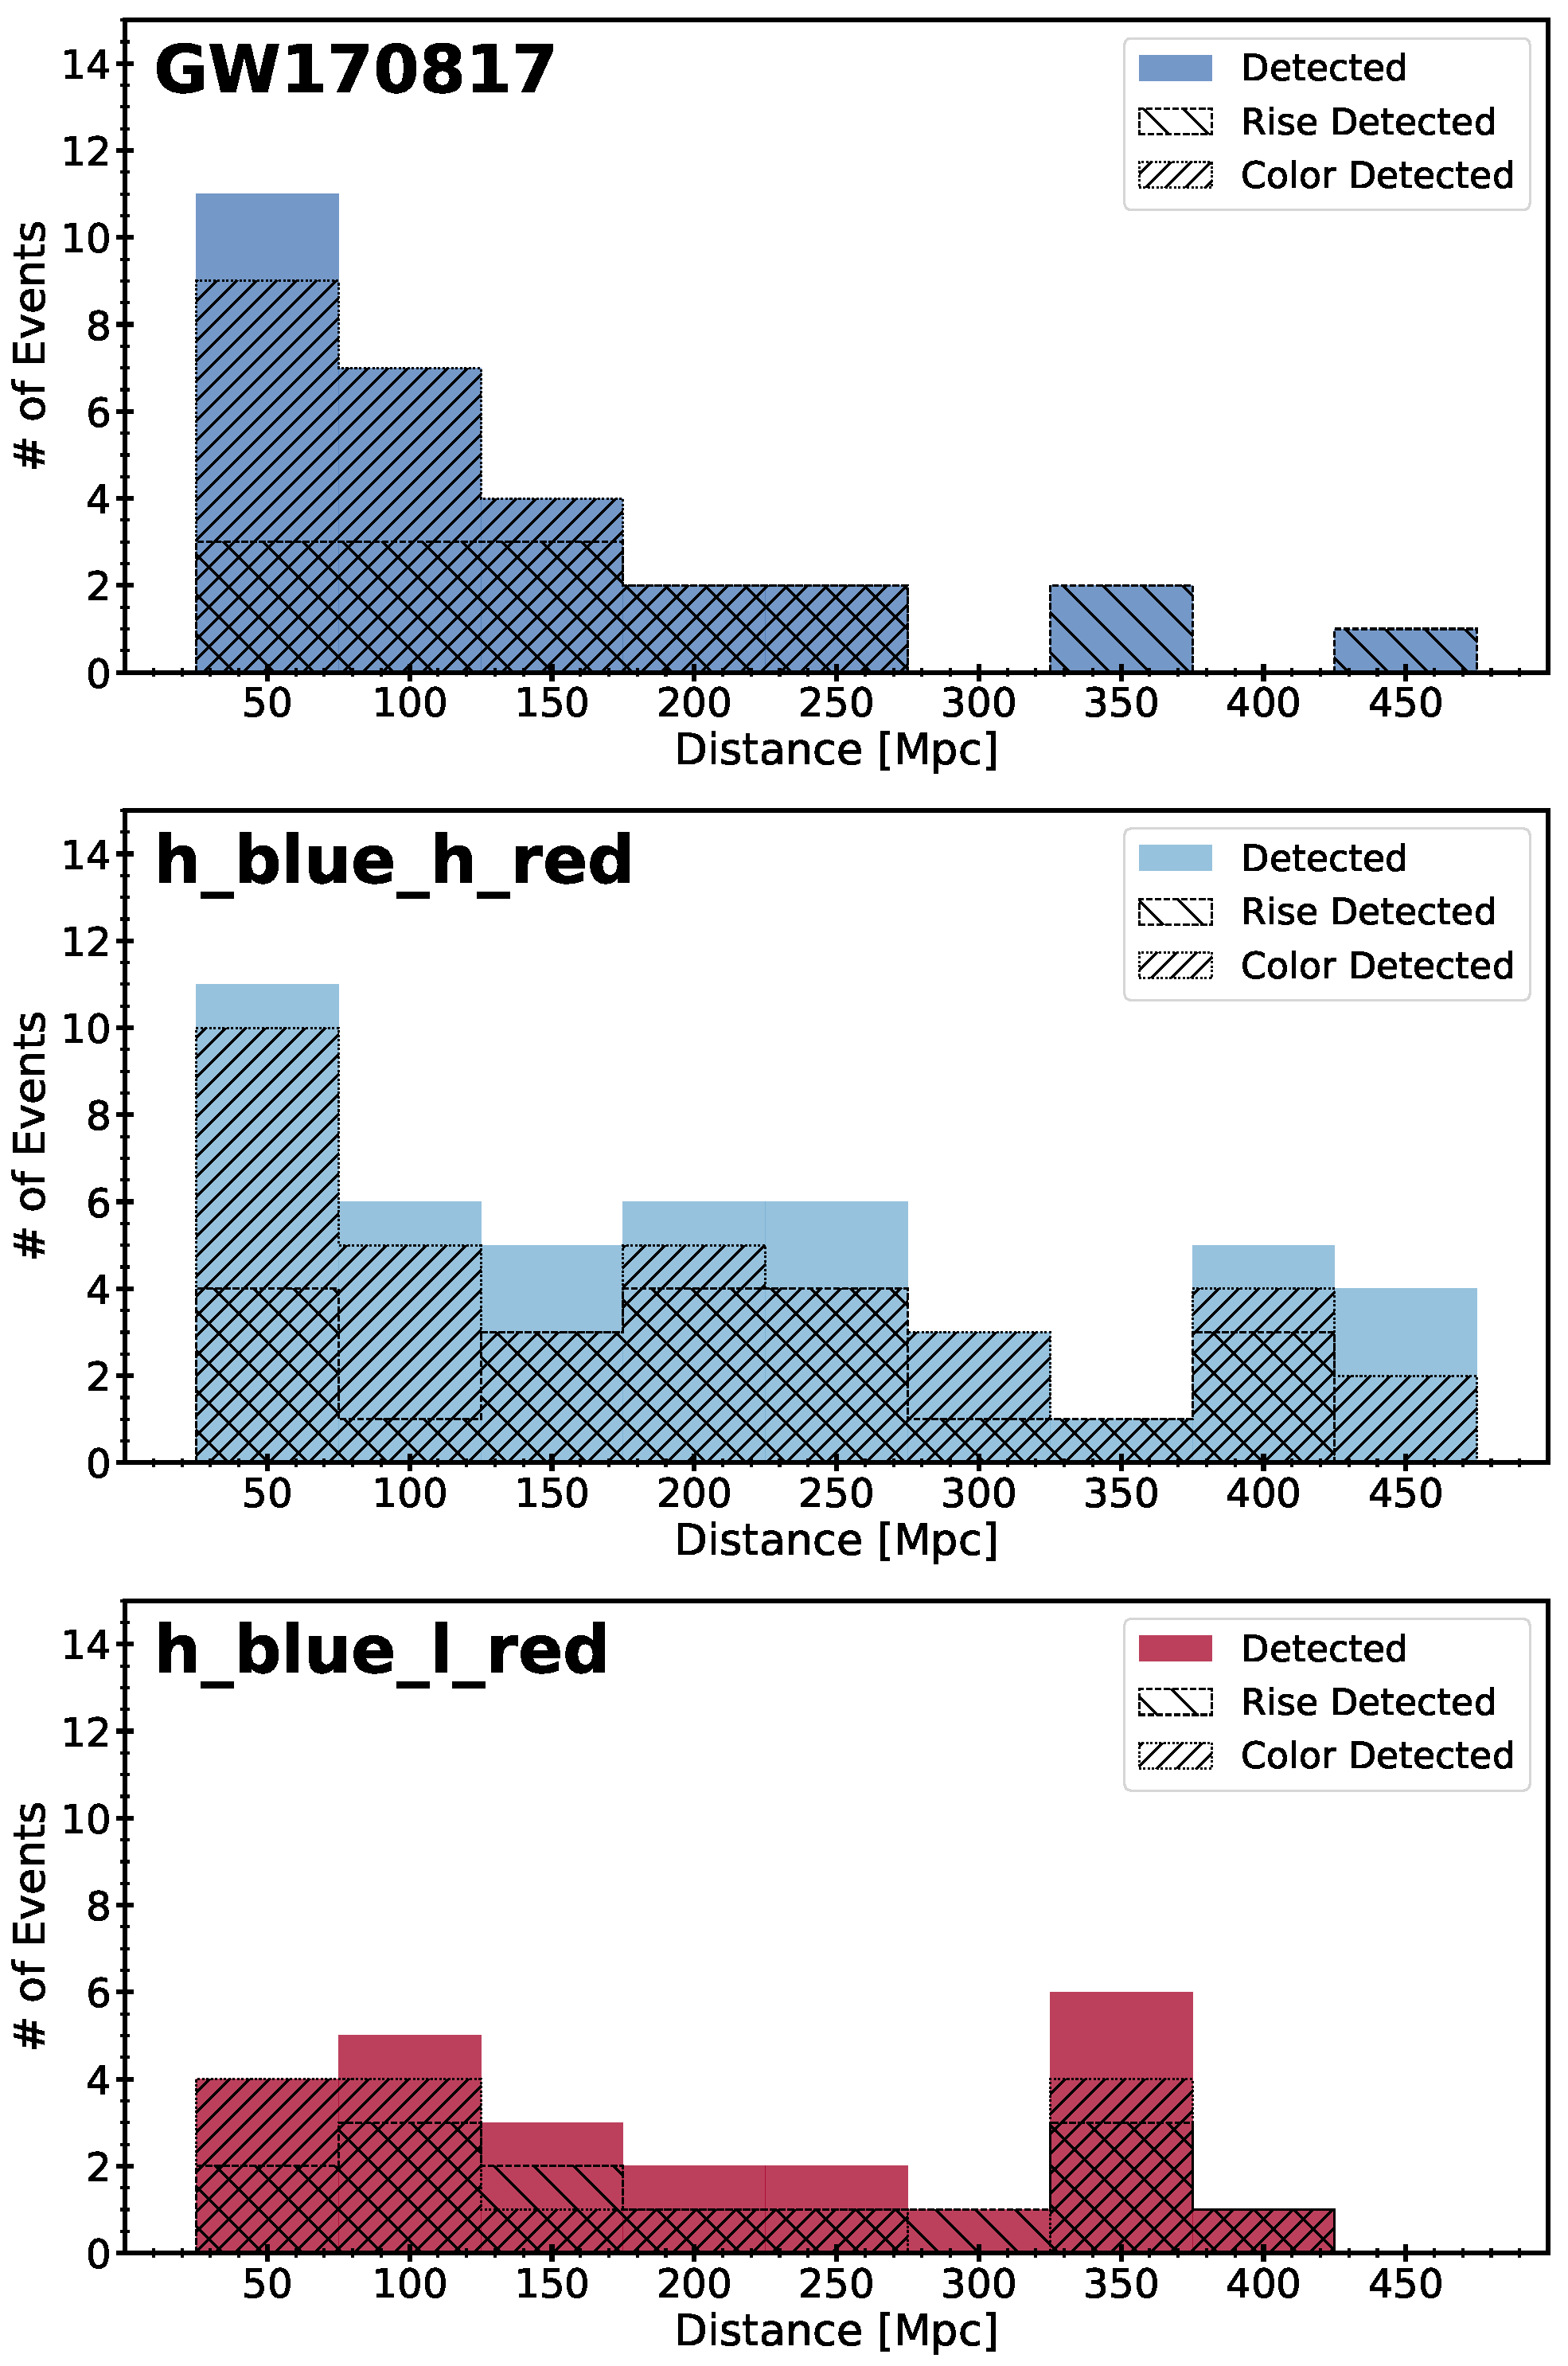
\includegraphics[width=0.7\textwidth]{./figs/chapter6/f1.pdf}}
\caption{\singlespace Histograms showing the number of detections as a function of model and distance, for those models that are detected. We note that as a result of the cadence of the LSST main survey we are not always able to obtain crucial information about the rise and color.}
\label{fig:ch6_eff_hist}
\end{center}
\end{figure}

Numbers of each value. Discuss plot.

Timing of detections and ability to detect early and late

\begin{figure}[!t]
\begin{center}
\hspace*{-0.1in}
\scalebox{1.}
{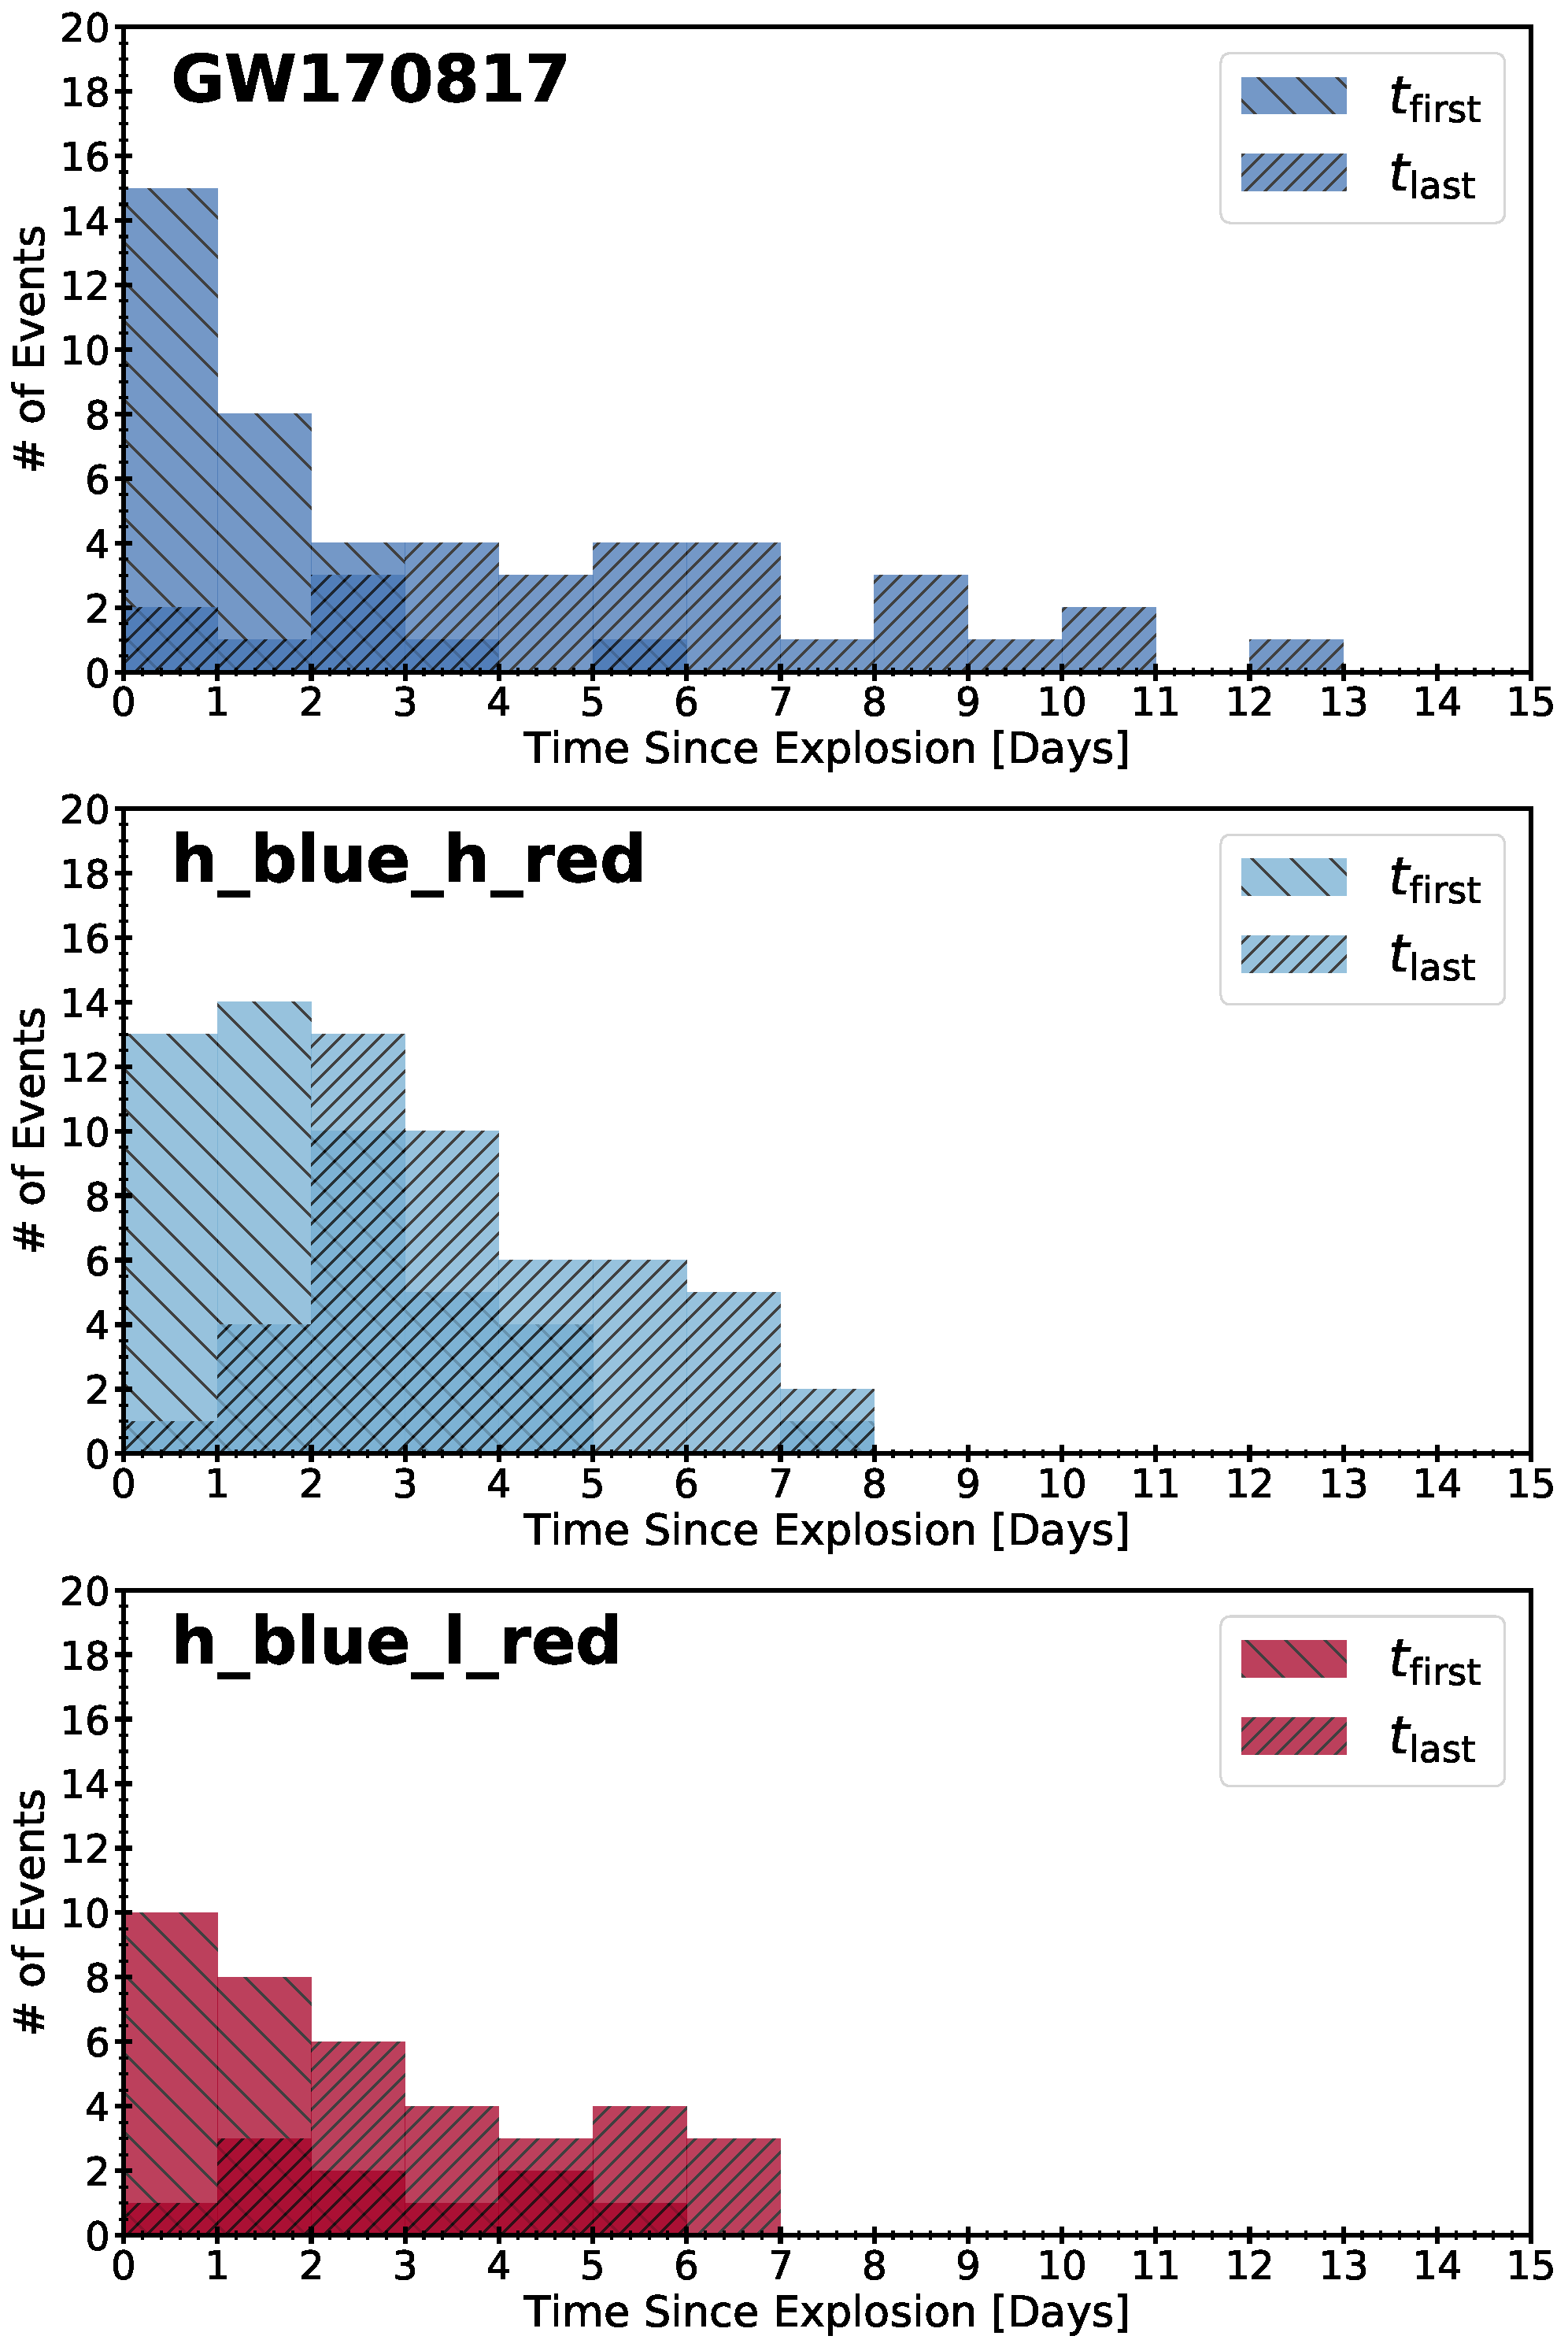
\includegraphics[width=0.7\textwidth]{./figs/chapter6/f2.pdf}}
\caption{\singlespace Histogram of events as a function of time to first or last detection. As with \Cref{fig:ch6_eff_hist}, we only plot those models that are detected. The LSST main cadence is only able to track a limited number of events out to longer times than \apx~a few days. This combined with the poor rise and color constraints shown in \Cref{fig:ch6_eff_hist} means that kilonovae detected in the LSST main survey will be difficult to detect and characterize.}
\label{fig:ch6_t_hist}
\end{center}
\end{figure}

Efficiencies. Discuss plot.

\begin{figure}[!t]
\begin{center}
\hspace*{-0.1in}
\scalebox{1.}
{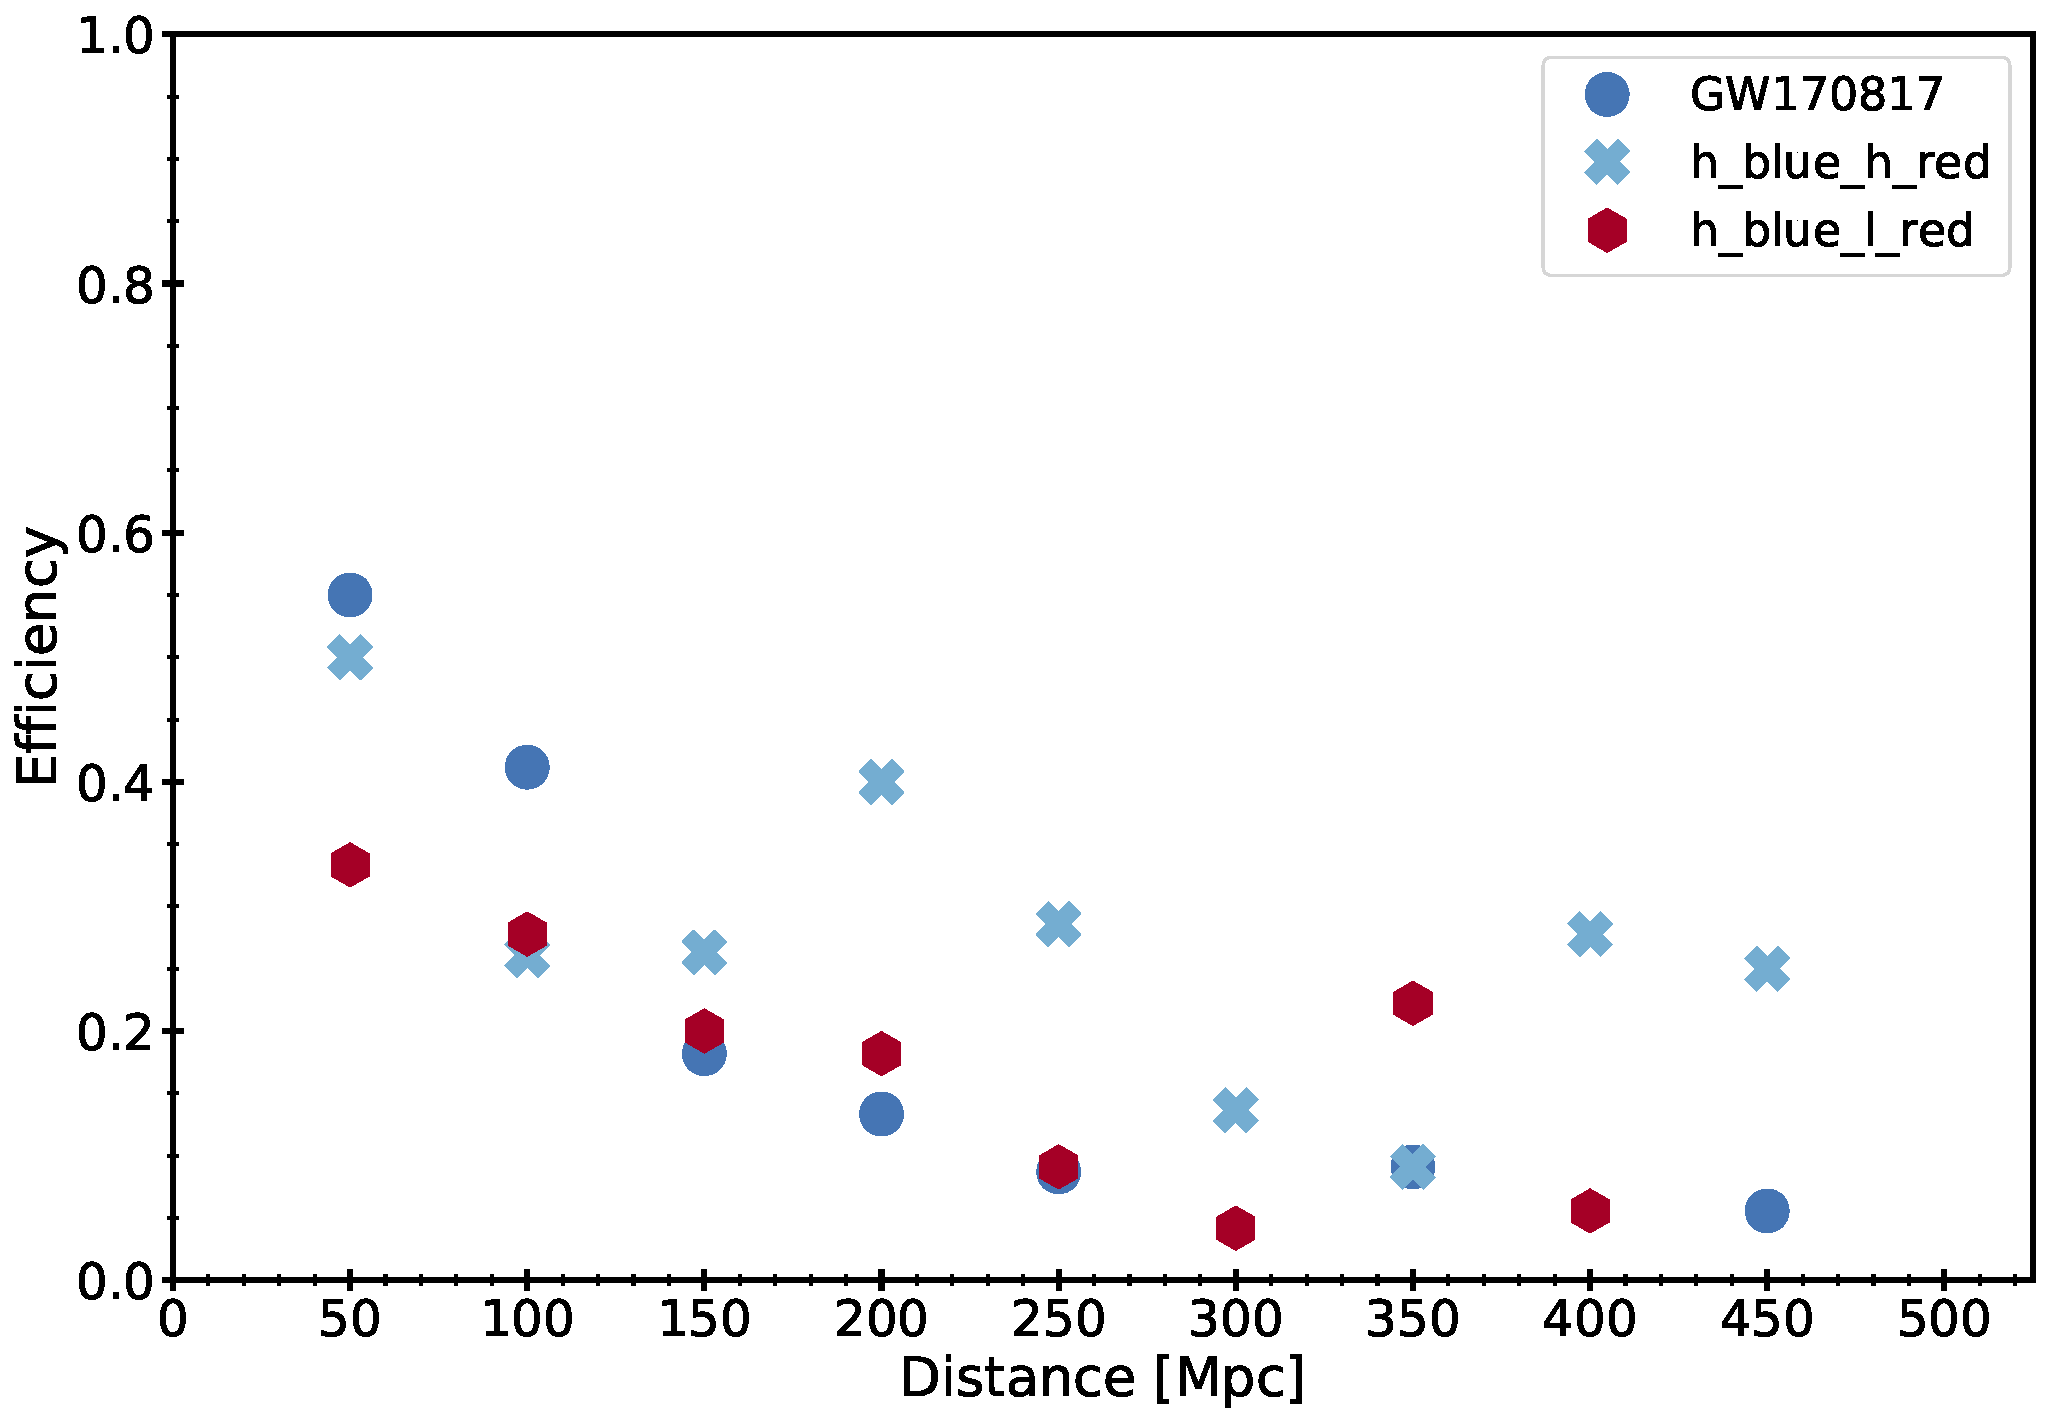
\includegraphics[width=0.9\textwidth]{./figs/chapter6/f3.pdf}}
\caption{\singlespace Detection efficiency as a function of distance for each of the detected models. As expected, the efficiency is high (\apx 60\%) for nearby sources ($D_L \apx 50$~Mpc), but rapidly tapers off to \apx10\% at the edge of the LIGO BNS detection range $(D_L \gtrsim 400$~Mpc).}
\label{fig:ch6_dist_eff}
\end{center}
\end{figure}

Expected rate and calculation

Implications

\subsection{Results from SNANA}
\label{sec:ch6_too_results}
Criteria same as used on LC from OpSim.

Same issue with models not being detected in standard 30s exposures. 

\begin{figure}[!t]
\begin{center}
\hspace*{-0.1in}
\scalebox{1.}
{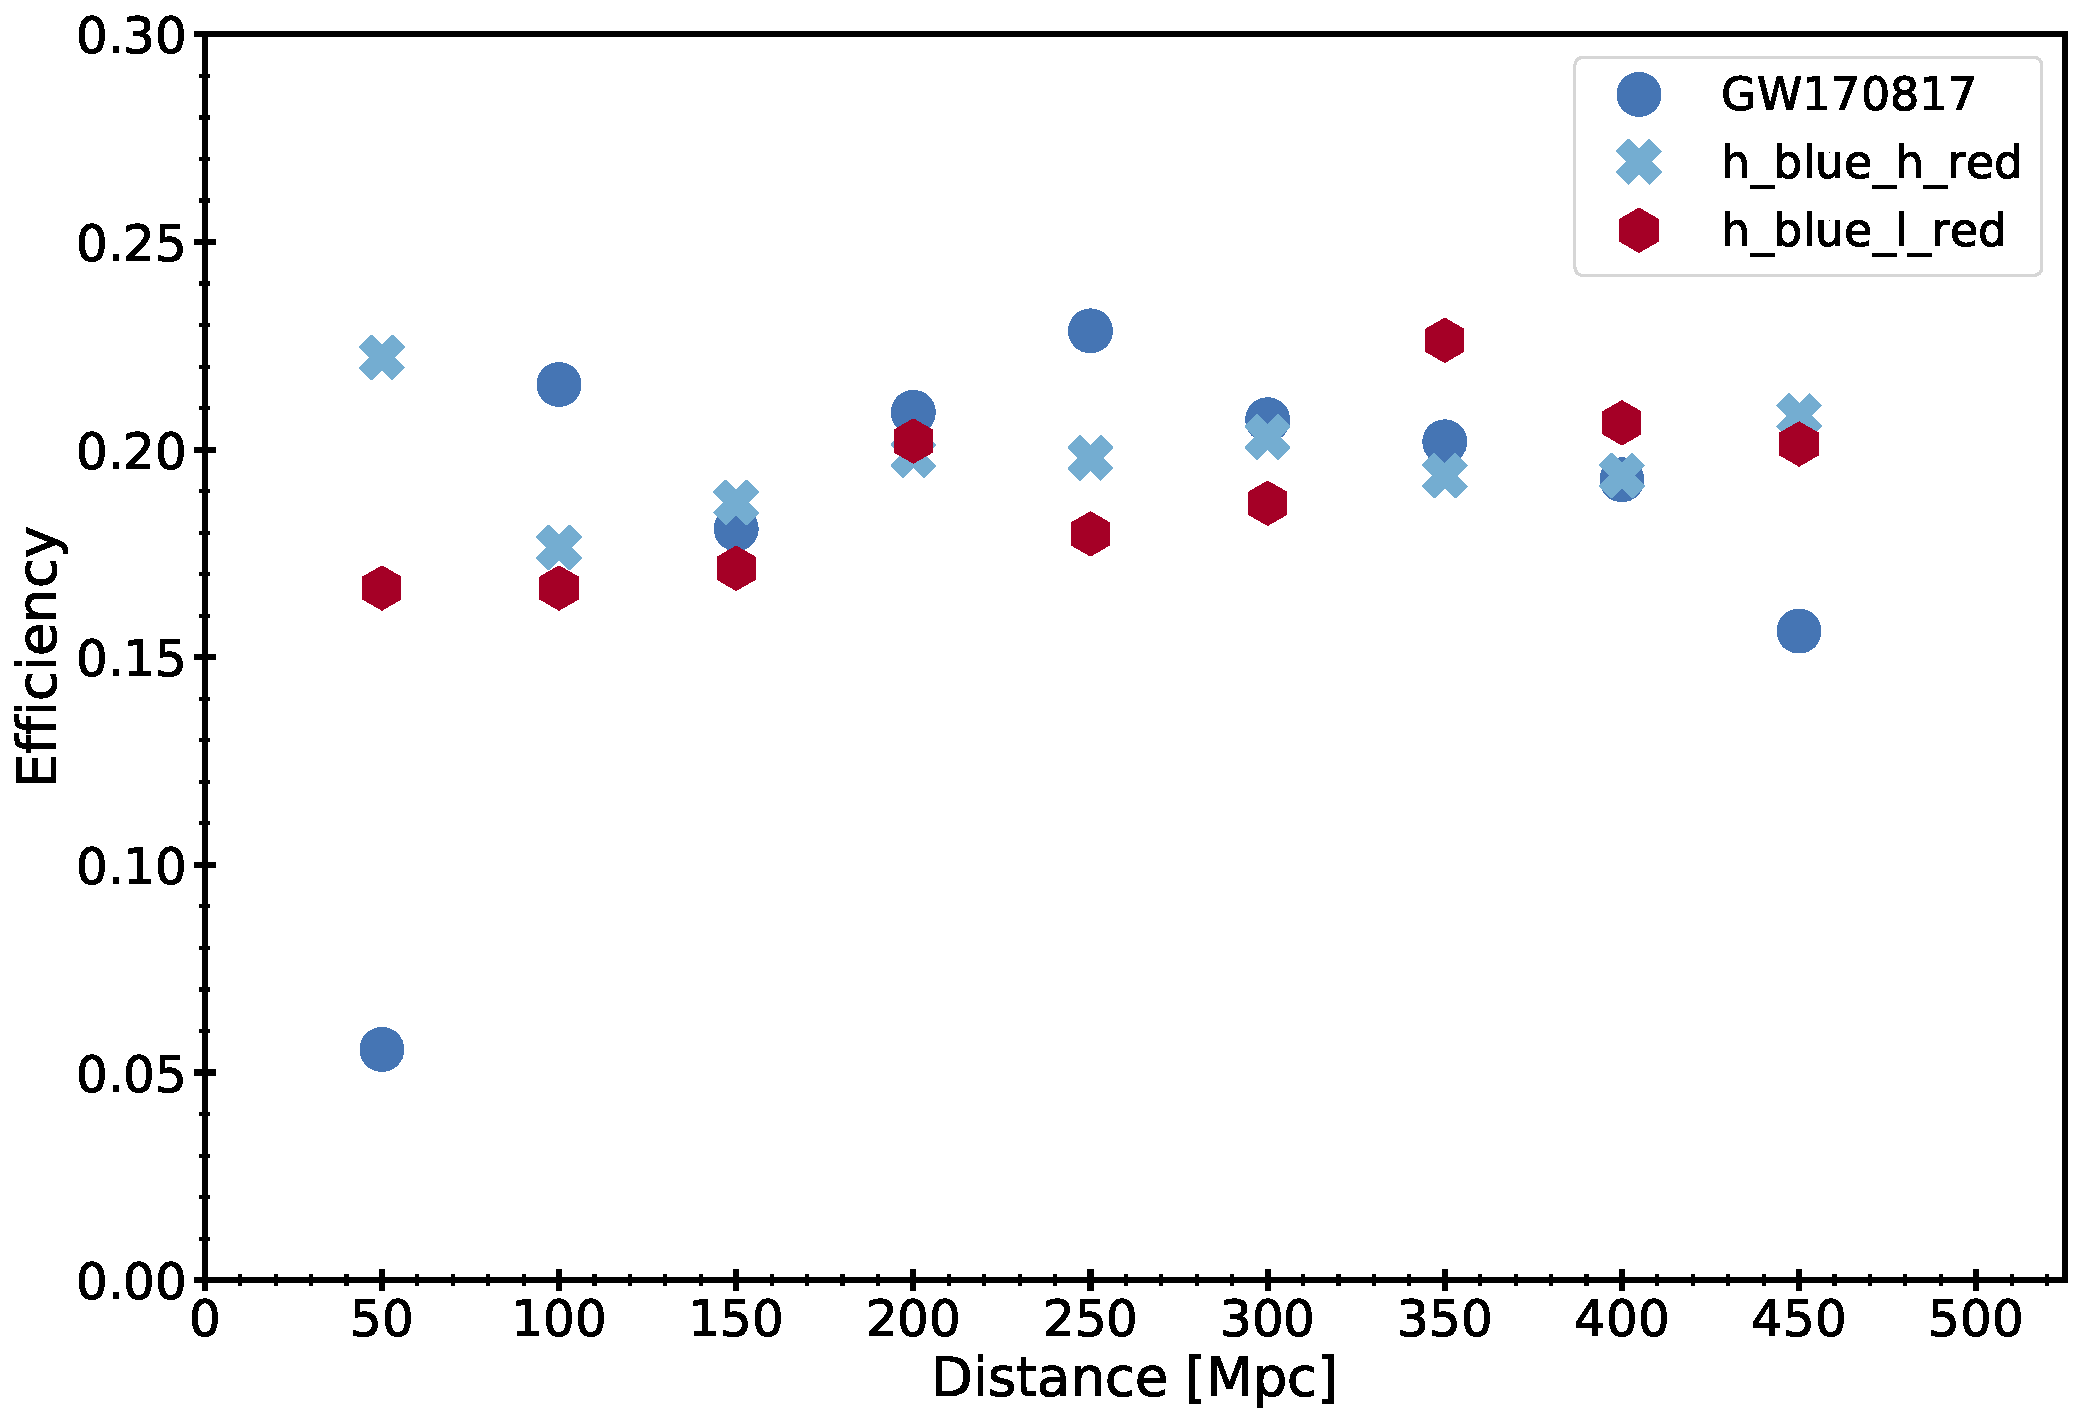
\includegraphics[width=0.9\textwidth]{./figs/chapter6/f5.pdf}}
\caption{\singlespace Efficiency of our ToO searches as a function of distance. The numbers plotted here are relative to the total number of injected sources (i.e., including models not detected). The {\it per model} detection efficiency is 100\% for the bright KN models plotted. The efficiency curve is flat as a function of distance indicating that ToO efforts with LSST can be effective out to the maximal LIGO BNS detection distance.}
\label{fig:ch6_dist_eff}
\end{center}
\end{figure}

Discuss plot. Stress that this is relative to all models injected. Efficiency for the bright models is 100\%. 0\% for faint models.

Effect of Start Time

\begin{figure}[!t]
\begin{center}
\hspace*{-0.1in}
\scalebox{1.}
{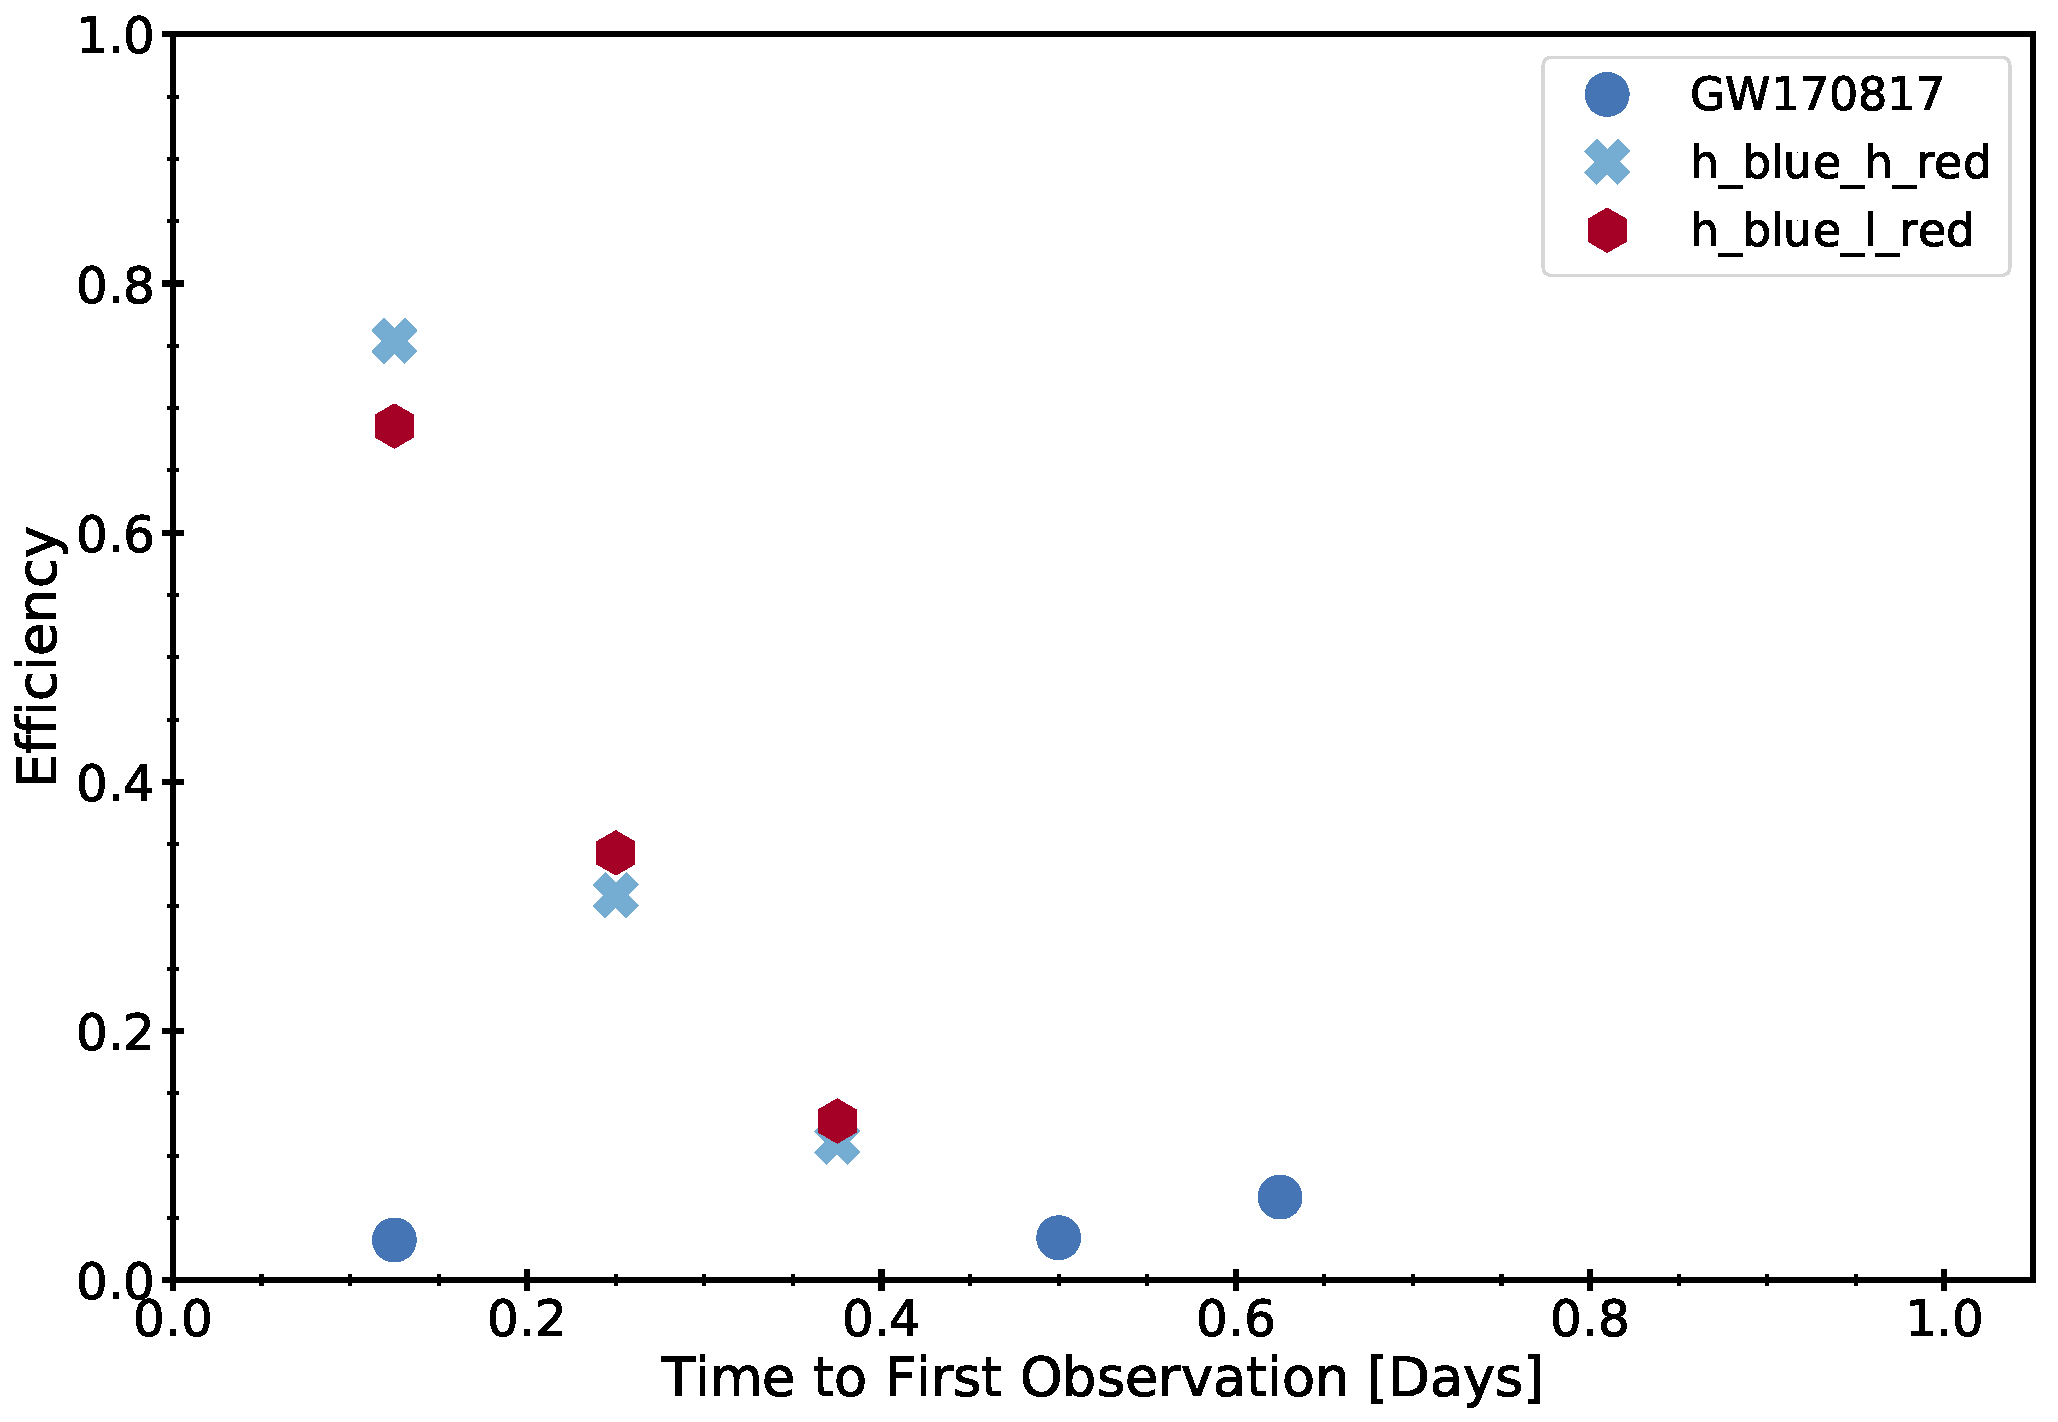
\includegraphics[width=0.9\textwidth]{./figs/chapter6/f6.pdf}}
\caption{\singlespace Efficiency of our ToO searches to detect brightening in the kilonova light curve in at least one filter as a function of starting time. The efficiency here is computed relative to the number of detected sources in a given time bin. There is a sharp drop off in efficiency after just a few hours. This efficiency drops to 0 under all observing scenarios when just a single epoch is obtained on the first night.}
\label{fig:ch6_dist_eff}
\end{center}
\end{figure}

discuss plot. No effect on detection or ability to detect rise. 

Effect of truncating time investment. None Really.

\section{Discussion and Conclusion}
\label{sec:ch6_conc}
We have done some LSST stuff. Major takeaway. LSST is good at ToO for bright KN. OpSim is okay at finding things over 10 years but unlikely to be associated with LIGO events.

Base exposures can only detect brightest novels. ToO needs to go deeper. Intermediate mass component possibly essential to GW170817 visibility.

Main survey summary

ToO summary

LSST must be involved in direct GW follow-up, well matched and won't find many in main survey in a usable sense.

%NO BIB INFO